\chapter{GATESIM METHODOLOGIES}
\label{chap:methodologies.tex}

Different methodologies could be adopted for netlist simulation and verification. The first step would be to obtain the test vector stimulus to the netlist. One approach could be to reuse the RTL testbench around the netlist. Another approach could be to replace only a portion of circuit with netlist in the existing RTL verification environment.

Another approach could be to capture test vectors from RTL simulation followed by applying it on corresponding netlist simulations. In such an approach comparison could be done between RTL behaviour stored as captured test vectores with that of netlist simulation.  In AMD, gatesim verification is accomplished by one such approach. Over the years, two different approaches were adopted for test vector capture and stimulus application. These are now called as Early Dual-Sim method and Co-sim based Gatesim method. Due to its many shortcomings, the early dual sim method was discontinued over Co-sim based Gatesim method. Co-sim based Gatesim is the current de-facto method for gate level simulations in AMD.


\section{EARLY DUAL-SIM METHODOLOGY}
Early method for gate level simulation was a dual-sim or simulation-after-simulation approach. Here RTL simulation was done initially with test bench components. The test vectors for gatesims were generated during this RTL simulation using ``\$display'' or VCD (value change dump). During netlist simulation, these test vectors were used as stimulus and comparison was done with the RTL output vectors. ~\figurename{~\ref{fig:early.eps}} shows the simulation flow. % Meera : 1. Figure x, 2. Have some good diagrams
%Naren: need this para re-write with references to figure

%\figurename{} 
\begin{figure}[H]
\centering
\includegraphics[width=4in, height=3.5in]{./figures/early.eps}
\caption{Early Dual-Sim Flow}
\label{fig:early.eps}
\end{figure}

This dual-sim approach is widely used across industry due to its many advantages. The main advantage of sim after sim is that it had the best simulation performance with least compute requirements. However the earlier implementation of this method had multiple disadvantages which became more prevalent with increasing design complexity.

\paragraph{Issues:}The main issue with earlier implementation of dual sim methodology was the huge disk space requirement. Vector files were text files which had cycle based information of stimulus. These files were large and simulation performance was also affected by disk input/output accesses. Another shortcoming of this methodology was that when stimulus was converted to cycle based information, inherent sampling errors were introduced, which were themselves causing simulation mismatches when compared with RTL simulations.

 
 With increasing design complexity, the disk-space requirements became too high that the method could no longer be sustained and a new co-simulation based approach was adopted instead.





\section{CO-SIM BASED GATESIM METHODOLOGY}
 Cosim-based approach was conceived to solve some problems that existed with dual-sim approach. To its advantage, the new approach enabled easy debug while maintaining consistent input vectors. It also made results comparision and debug easier.  ~\figurename{~\ref{fig:cosim.ps}} shows how stimulus is appiled to netlist and comparison of output is done in cosim method.
 
\begin{figure}[h!]
\centering
\includegraphics[width=4in, height=3.5in]{./figures/cosim.ps}
\caption{Co-sim Based Gatesim}
\label{fig:cosim.ps}
\end{figure}


 In Cosim methodology, a single combined simulation with behavioral RTL design and netlist with all of the required RTL stimulus components is made. In this simulation, behavioral RTL and gate models are run in lock-step with their inputs tied and the comparison of the behavioral RTL and gate outputs is done ``on the fly''. ~\figurename{~\ref{fig:cosim_flow.eps}} shows cosim flow.




%\figurename{} 
\begin{figure}[H]
\centering
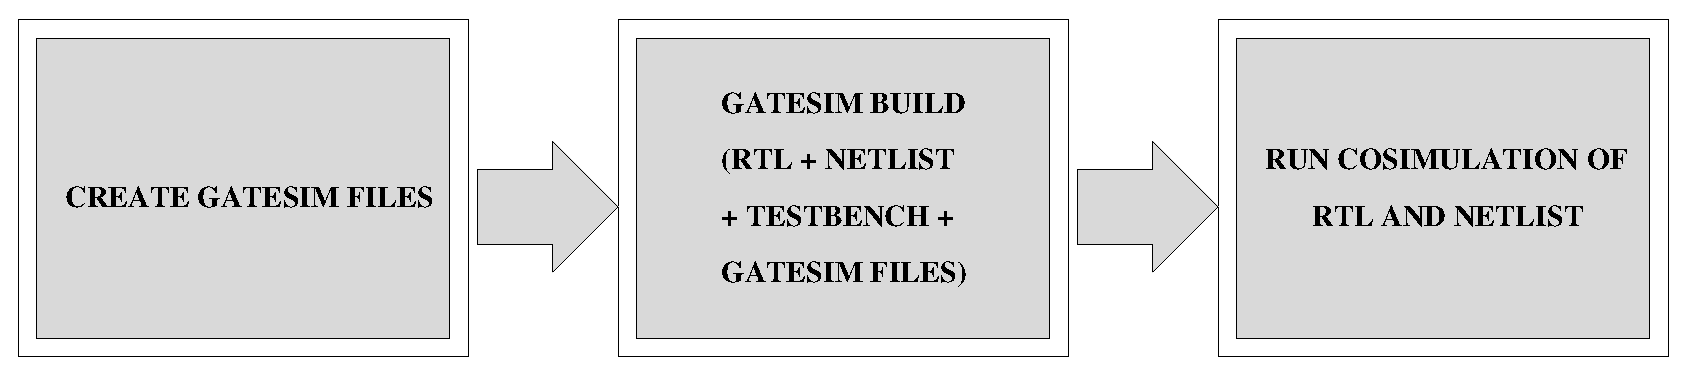
\includegraphics[width=4in, height=1.5in]{./figures/cosim_flow.ps}
\caption{Co-sim Based Gatesim Flow}
\label{fig:cosim_flow.eps}
\end{figure}

Major steps involved in this flow are:

\begin{enumerate}
	\item \emph{\bf Getting gatesim files}

	Input to gatesims are files obtained from LEC tools. These file include the netlist file, files holding information regarding IO/Register mapping, gate defines, compare enables and testbench force files. These inputs from LEC stage are processed by a set of scripts for developing intermediate files which are needed by cosim build infrastructure. These files are called gatesim files and these verilog files are:
	\begin{itemize}
		\item File which contain top level module that connects the behavioral RTL signals to the corresponding gate signals.
		\item Test bench compare files that contain the verilog compare code used to compare the outputs and register mappings.
		\item Force files that contain all the force/release/assign commands for the gates corresponding to RTL force/release/assign statements.
	\end{itemize}

	\item \emph{\bf Getting gatesim build} 

	Next stage is to enable a build structure supporting the co simulation of RTL and Netlist. The build infrastructure will include the following:
	\begin{itemize}
		\item[-]Netlist
		\item[-]RTL
		\item[-]Test bench
		\item[-]Gatesim files
	\end{itemize}

	\item \emph{\bf Run cosimulation of RTL and netlist}

	Finally, run cosimulation. Output files include $<$testname$>$.out which contains the simulation log of the entire test and $<$test name$>$.fsdb (if wave form dump enabled).
\end{enumerate}


As the netlist stimulus is obtained from a live RTL instead if from storage files, cosim based gatesim overcame the biggest limitation associated with dual-sim. Along with some good set of scripts aiding testbench generation and force generation, this method became the standard method for gatesims ever since.

\subsection {ISSUES WITH CURRENT CO-SIM METHOD}

Co-sim based Gatesim overcame all the known limitation associated with early approach but brought in new set of limitations as design complexity grew. Of those the important limitations were:

\begin{itemize}
	\item[-]Larger turn-around time (run, debug cycle).
	\item[-]Limitation on size of netlist (indirect cause due to larger build and run time).
\end{itemize}

\subsubsection {Simulation performance analysis}
Experiments showed that the simulation performance of gatesim was affected sometimes as low as 10\% with respect to its counterpart RTL simulations. This indicates that:

\begin{itemize}
	\item[-]RTL Simulations contribute major to simulation preformance than netlist.
	\item[-]Simulator spends more time in simulating RTL and verification components than netlist.
\end{itemize}

On further investigation it became clear that RTL simulation, which is simulated redundantly for the sole purpose of generating test vectors influences the simulation performance greatly. Such complex SOC design has multitude of Verification components in different programming languages including C, C++, SVTB, OVA, SVA and that these verification components take a big share of simulation cycles and have negative effect on simulation performance.

Evidently it was not an appropriate use of compute resources by having live RTL simulation every time, for the sole purpose of test vector generation. The analysis provides convincing evidence for us to attempt changes in existing cosim-based methodology.
